\subsection{Node2vec}
In this paper we will look at graph embedding as a way to find structural similarity between nodes in a graph, specifically node embedding. This is done using the implementation in “Node2vec: Scalable Feature Learning for Networks” by Aditya Grover and Jure Leskovec \cite{Node2vec}. They present an algorithm called node2vec for efficient feature learning for nodes in networks. This is done by mapping nodes to a vector representation of their features, that try to preserve local networks of neighborhood nodes and communities, using a random walk approach to generate a nodes neighborhood network.

Node2vec makes use of the word2vec skip-gram model to train a model for embedding the nodes.
The idea behind the model is that given a specific word in a sentence, look at the window around it, and pick a random word within the window. As output we get for each word, the probability for an associated word being the randomly chosen one \cite{Word2vec}.
The model is trained by feeding it pairs of words from sentences, sliding the window across a sentence and picking random words for each specific word, training the model on how often each word pairing shows up. An example can be seen in \autoref{fig:wordpair_example}.

\begin{figure}[H]
\centering
  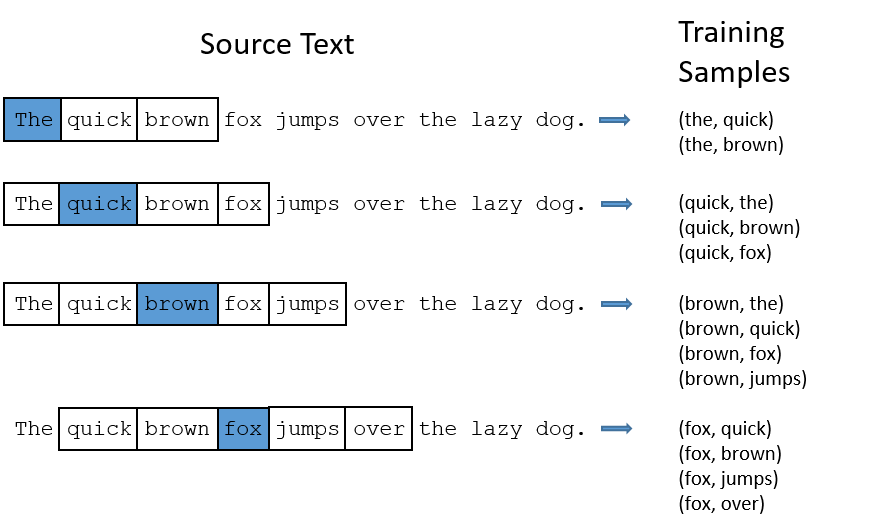
\includegraphics[scale=0.6]{Article/figures/training_data.png}
  \caption{Example of word pair sample generation \cite{Word2vec}}
  \label{fig:wordpair_example}
\end{figure}

First a vocabulary $V$ is created, that consist of all unique words found in the sentences. The input is a single word, represented as a one-hot encoding, of size $|V|$. The size of the hidden layer is the number of features or dimensions $d$ that we want to learn. Lastly the output layer is a vector of size $|V|$, containing the probability for each word in our vocabulary being the randomly chosen word. An example of the network is shown in \autoref{fig:skip-gram_example}.

\begin{figure}[H]
\centering
  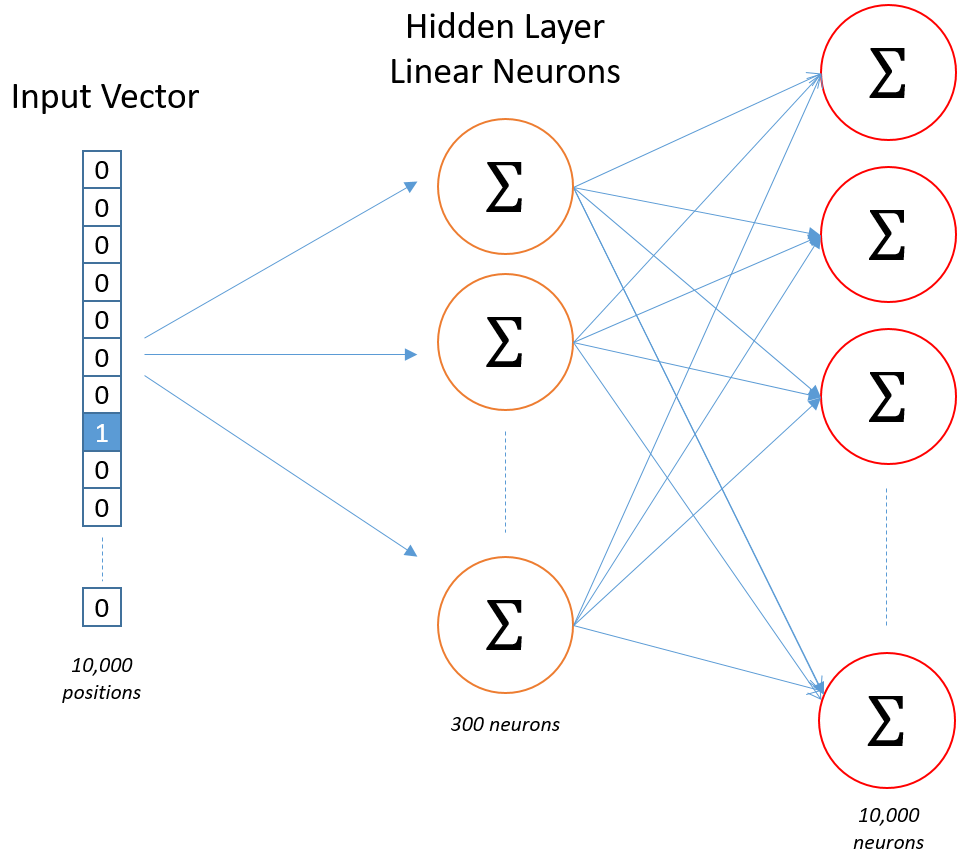
\includegraphics[width=\linewidth]{Article/figures/skip_gram_net_arch.png}
  \caption{Example of the skip-gram network \cite{Word2vec}}
  \label{fig:skip-gram_example}
\end{figure}

Once trained is done, instead of using the model for further calculations, the model is discarded and only the weights of the hidden layer is kept. These weights are then what is used as our embedding vectors. Giving us $V$ vectors of size $d$.


In article \cite{Node2vec} feature learning is explained in further details where for every source node $u \in V$, $N_s (u) \subset V$ is defined as a network neighborhood of a node $u$, generated through a sampling strategy $S$.

Feature learning methods based on the skip-gram model were developed within the context of natural languages. Text have a linear nature in form of sentences and the notion of a neighborhood can in that case easily be defined by sliding the window across the sentence. Networks are not linear and therefor a richer notion of a nodes neighborhood is needed. For this they propose a random walk, that samples different neighborhoods $N_s (u)$ for a given source node $u$, and can have very different structures depending on the sampling strategy $S$ used.

Thus given a graph and a source node, we want to sample its neighborhood, the size of the neighborhood set $N_s(u)$ is constrained to $k$ nodes and will sample multiple neighborhood sets for a single node $u$ using a sampling strategy $S$.

There is in general two sampling-strategies for generating neighborhood sets \cite{Node2vec}. The first one is a Breadth-first sampling (BFS) strategy, where a nodes neighborhood is restricted to nodes which are immediate neighbors to the node, finding the immediate community that the node is part of. This gives us a microscopic view of the neighborhood and is therefor good for finding structural equivalence.

The second one is Depth-first sampling (DFS) strategy, where a nodes neighborhood consist of nodes sampled at an increasing distance from the node, giving a bigger view of the structure and its differences. This gives us a macro-view of the neighborhood, which is essential for inferring communities based on homophily.

Networks commonly contains both behaviors, where some nodes exhibit homophily while others reflect structural equivalence, thus a sampling strategy that can sample both behaviors is needed.

For this \cite{Node2vec} formulate a sampling strategy $S$, which is a biased random walk procedure, that can explore in a BFS as well as DFS approach.

Given a source node $u$, simulate a random walk of length $l$. Let $c_i$ be the i'th node in the walk, starting with $c_o = u$. Nodes $c_i$ are then generated by the distribution given in \autoref{EQ:n2v_distribution}.

\begin{equation}\label{EQ:n2v_distribution}
P(c_i = x | c_{i-1} = v) = 
\begin{cases} 
	\frac{\pi_{vx}}{Z}  \; \text{if} \: (v,x) \in E \\
	0 \; \text{otherwise}
\end{cases}
\end{equation}

where $\pi_{vx}$ is the unnormalized transition probability between node $v$ and $x$, and $Z$ is the normalizing constant.

A $2^{nd}$ order random walk is defined, with two parameters $p$ and $q$, which helps guide the walk.

\begin{figure}[H]
\centering
  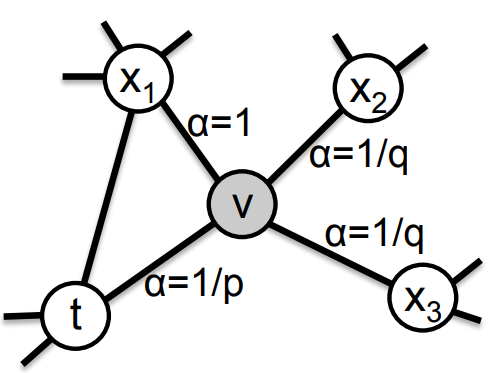
\includegraphics[scale=0.5]{Article/figures/randomwalkexample.png}
  \caption{Random walk example of node2vec \cite{Node2vec}}
  \label{fig:n2v_randomwalk}
\end{figure}

As an example, look at figure \autoref{fig:n2v_randomwalk} and consider a random walk that have just travelled the edge $(t, v)$ and which now resides at node $v$. The walker will then have to decide on the next step to take. It then evaluates the transition probabilities $\pi_{vx}$ on edges $(v,x)$ leading from node $v$. The unnormalized transition probability is set to $\pi_{vc} = \alpha_{pq} (t,x) \times w_{vx}$ where \autoref{EQ:n2v_transition_probability} applies.

\begin{equation}\label{EQ:n2v_transition_probability}
\alpha_{pq} (t,x) =
\begin{cases} 
	\frac{1}{p} \; \text{if} \:  d_{tx} = 0 \\
	1 \; \text{if} \: d_{tx} = 1 \\
	\frac{1}{q} \; \text{if} \: d_{tx} = 0
\end{cases}
\end{equation}

In \autoref{EQ:n2v_transition_probability} $d_{tx}$ denotes the shortest path distance between nodes $t$ and $x$. In this case $p$ and $q$ controls how fast the walker explores and leaves the neighborhood of a starting node $u$, allowing the walker to interpolate between the BFS and DFS sampling methods.

$p$ is the return parameter, and controls the likelihood of immediately revisiting a node in the walk. A high value ensures that you are less likely to sample an already visited node, encouraging exploration, whereas a low value will keep the walker close to a starting node $u$.

$q$ is the In-out parameter, and allows the search to differentiate between inward and outward nodes. A high value will keep the walker more biased towards a starting node $u$, obtaining a local view. Whereas a low value will make the walker more inclined to visit nodes further away from $u$, encouraging outward exploration.

Using the node2vec strategy, the transition probabilities for a network is calculated for each node depending on $p$ and $q$. A random walker then traverses the network, sampling a chosen amount of neighborhood(s) $N_s(u)$. These neighborhoods acts as the sentence given to the word2vec skip-gram model, learning the probabilities for the nodes being related to eachother and learning the embeddings for each node.
